\documentclass[xcolor={dvipsnames}]{beamer}
\usepackage[utf8]{inputenc}
\usepackage[english]{babel}
\usepackage{amsmath,amsfonts,amssymb, bm}
\usepackage{cancel}
\usepackage{graphics}
\usepackage{algorithm}
\usepackage{algpseudocode}
\usepackage{cancel}
\usepackage{booktabs}


\graphicspath{{figures/}} % Location of the graphics files
\usetheme{CambridgeUS}
\usecolortheme{dolphin}
\usefonttheme{structuresmallcapsserif}
\setbeamertemplate{blocks}[rounded][shadow=false]
\addtobeamertemplate{navigation symbols}{}{%
    \usebeamerfont{footline}%
    \usebeamercolor[fg]{footline}%
    \hspace{1em}%
    \insertframenumber/\inserttotalframenumber
}

\AtBeginSection[]{
  \begin{frame}
  \vfill
  \centering

  \begin{beamercolorbox}[sep=8pt,center,shadow=false,rounded=true]{title}
    \usebeamerfont{title}\insertsectionhead\par%
  \end{beamercolorbox}
  \vfill
  \end{frame}
}

% \newcommand{\red}[1]{\color{red} #1 \color{black}}
% \newcommand{\green}[1]{\color{OliveGreen} #1 \color{black}}
% \newcommand{\control}[1]{\color{blue} #1 \color{black}}
% \newcommand{\donnee}[1]{\color{BurntOrange} #1 \color{black}}

% \newcommand{\cv}{\rightarrow}
% \newcommand{\cvlaw}{\xrightarrow{\mathcal{L}}}
% \newcommand{\Then}{\Rightarrow}
% \newcommand{\prodd}[2]{\langle #1,#2 \rangle}
% \newcommand{\R}{\mathbb{R}}
% \newcommand{\N}{\mathbb{N}}
% \newcommand{\E}[1]{\mathbb{E}\left[#1\right]}
% \newcommand{\normal}[2]{\mathcal{N}\left(#1, #2 \right)}
% \newcommand{\cvprob}{\xrightarrow{P}}
% \newcommand{\cvas}{\xrightarrow{a.s.}}
% \newcommand{\lac}{\left\{}
% \newcommand{\rac}{\right\}}
% \newcommand{\xd}{\bm{X}}
% \newcommand{\yd}{\bm{Y}}

% \newcommand{\predInterv}[1]{\mathcal{I}_{pred}(#1)}
% \newcommand{\thetah}{\hat{\theta}}
% \newcommand{\rtparam}[1]{\red{\theta^{(T)}_{#1}}}
% \newcommand{\rlparam}[1]{\red{\theta^{(L)}_{#1}}}
% \newcommand{\rdparam}[1]{\red{\theta^{(D)}_{#1}}}
% \newcommand{\rparam}[1]{\red{\theta^{(#1)}}}
% \newcommand{\var}[2]{#1^{(#2)}}

% \newcommand{\Yx}{\var{Y}{x}}
% \newcommand{\Yz}{\var{Y}{z}}
% \newcommand{\Xp}[2]{\var{X}{#1}_{#2}}
% \newcommand{\yx}{\var{y}{x}}
% \newcommand{\yz}{\var{y}{z}}
% \newcommand{\xp}[2]{\var{x}{#1}_{#2}}
% \newcommand{\tparam}[1]{\theta^{(T)}_{#1}}
% \newcommand{\lparam}[1]{\theta^{(L)}_{#1}}
% \newcommand{\dparam}[1]{\theta^{(D)}_{#1}}
% \newcommand{\bY}{\bm{Y}}
% \newcommand{\bX}{\bm{X}}

% \newcommand{\logL}{\log \mathcal{L}}
% \newcommand{\Like}{\mathcal{L}}
% \newcommand{\Prob}{\mathbb{P}}
% \newcommand{\Cov}{\bm{\Sigma}}
% \newcommand{\hCov}{\hat{\bm{\Sigma}}}
% \newcommand{\Norm}{\mathcal{N}}

\title{Facebook}
\subtitle{Mixed effects models: Inference and Maximum Likelihood\\~\\

\includegraphics[height=1.5cm]{logo_x}

\includegraphics[height=1.5cm]{logo_inria}}
\institute{CMAP, Ecole Polytechnique}
\date{September 27th, 2017}

\begin{document}

\begin{frame}
\titlepage
\end{frame}

\begin{frame}
\frametitle{Plan}
\tableofcontents
\end{frame}




\section{Problem}

\begin{frame}
\frametitle{Notations}

\begin{itemize}
\item $\var{Z} = (\var{Z}_1,\dots,\var{Z}_N) \in \mathcal{Z} \subset \mathbb{R}^d, \var{Y} = (\var{Y}_1,\dots,\var{Y}_N) \in \mathcal{Y} \subset \mathbb{R}^d$ Random Variables
\item Measurable spaces with the associated incomplete and complete densities $p(y_i,\theta)$ and $p(y_i,z_i,\theta)$ where:
\begin{itemize}
  \item $y_i$ is observed
  \item $z_i$ is the individual parameter
  \item $\theta$ is the population parameter
\end{itemize}
\item Continuous, non linear and mixed effects models:
\begin{equation}
y_{i} = f(z_{i}) + \epsilon_i
\end{equation}
Where:
\begin{itemize}
  \item The structural model $f: \Theta \to \mathbb{R}$ is non linear and twice differentiable
  \item $\epsilon_i \sim \mathcal{N}(0,\sigma^2)$ and $\sigma \in \mathbb{R}$
  \item $z_i \sim \mathcal{N}(z_{pop},w^2)$ such that $z_i = z_{pop} + \eta_i$ with $\eta_i \sim \mathcal{N}(0,\omega^2)$
  \item $y_i | z_i \sim \mathcal{N}(f(z_i),\sigma^2)$
\end{itemize}
\item In our case $\theta = (z_{pop}, \omega, \sigma )$

\end{itemize}

\end{frame}

\begin{frame}
\frametitle{Maximum likelihood}

The goal is to compute the maximum likelihood estimate
\begin{equation}
\theta^{ML} = \arg \max \limits_{\theta \in \Theta} p(y,\theta)
\end{equation}

The EM algorithm (Dempster, Laird and Rubin) is an iterative algorithm that computes this quantity by maximizing an auxialiary quandity $Q: \Theta^2 \to \mathbb{R}$ at a given parameter estimate $\theta'$:
\begin{equation}
Q(\theta, \theta) = \mathbb{E}_{p(z|y,\theta')}\left[ \log p(y, z, \theta) \right]
\end{equation}

Unfortunately, in the framework of nonlinear mixed effects models, there is no explicit expression for the E-step since the relationship between observations y and individual parameters z is nonlinear so the expectation cannot be computed in closed form. Thus, we use a stochastic version of the EM.
\end{frame}



\section{Parameter Estimation: SAEM algorithm}

\begin{frame}
\frametitle{SAEM}
At a given $\theta^{k-1}$:
\begin{enumerate}
  \item $z_i^k \sim p(z_i|y_i,\theta^{k-1})$
  \item $Q^k(\theta) = Q^{k-1}(\theta)+ \gamma_k(\log p(y_i, z_i^k, \theta) - Q^{k-1}(\theta))$
  \item $\theta ^k = \arg \max \limits_{\theta \in \Theta} Q^k(\theta)$
\end{enumerate}


My goal being to accelerate this algorithm, three approaches have been taken yet:
\begin{itemize}
  \item Incremental/mini-batch strategies (see Neal $\&$ Hinton on the EM or F.Bach on the SGD)
  \item Faster MCMC dynamics (SG-MCMC based on an ITO diffusion, see for instance MALA based on a Langevin diffusion)
  \item Efficient proposal for a Metropolis Hastings algorithm based on a Laplace Approximation of the incomplete log likelihood $\log p(y,\theta)$
\end{itemize}


\end{frame}



\section{Inference: MCMC}

\begin{frame}
\frametitle{Inference: MCMC}

\begin{itemize}
\item First Order Conditional Estimation Method
  \begin{enumerate}
    \item Laplace Approximation of the incomplete likelihood around the MAP ($z_{i,MAP} = \arg \max \limits_{z} p(z_i|y_i,\theta)$)
    \begin{align}
    p(y_i,\theta) & = \int{p(y_i,z_i,\theta) dz_i} = \int{e^{\log p(y_i,z_i,\theta)} dz_i}\\
    & \approx e^{\log p(y_i,z_{i,MAP},\theta)} \sqrt{\frac{(2\pi)^p}{|-\nabla^2\log p(y_i,z_{i,MAP},\theta)|}}
    \end{align}
    \item Approximation of the posterior
    \begin{align}
    -2 \log p(y_i,\theta) = & \underbrace{-p \log(2\pi) +\log(|-\nabla^2\log p(y_i,z_{i,MAP},\theta)|)}_{\approx -2\log p(z_{i,MAP}|y_i,\theta)} \\
    & -2\log p(y_i,z_{i,MAP},\theta)
    \end{align}
  \end{enumerate} 
\item Equivalent to linearizing the structural model $f$ around the MAP:
\begin{align}
y_i \approx z_{i,MAP} + (z_i - z_{i,MAP})\nabla_{z_i} f(z_{i,MAP}) + \epsilon_i \implies z_i|y_i \sim \mathcal{N}(\mu, \Gamma)
\end{align}



\end{itemize}

\end{frame}




\section{Applications}

\begin{frame}
\frametitle{PK-PD datasets}

\begin{itemize}
\item The data comes from 37 winter wheat experiments carried out between 1990
and 1996 on commercial farms near Paris, France. Each experiment was from a different site.
\item Each experiment consisted of five to eight different nitrogen fertiliser rates, for a total of 224 nitrogen treatments. Nitrogen fertilizer was applied in two applications during the growing season. For each nitrogen treatment, grain yield (adjusted to 150 g.kg-1 grain moisture content) was measured.
\item In this problem the sites are denoted by the index "i" and are the individuals in the dataset, the predictor is the dosage, the response is the grain yield and the covariate is the soil nitrogen
\end{itemize}
\end{frame}

\begin{frame}
\frametitle{Comparison}

\begin{itemize}
\item New independent proposal. At a given iteration $k$:

  \begin{equation}
  z_i^k \sim \mathcal{N}(z_{i,MAP}, |-\nabla^2\log p(y_i,z_{i,MAP},\theta)|)
  \end{equation}
\item Comparison of the MCMC properties with:
\begin{itemize}
  \item Random Walk Metropolis (proposal $\mathcal{N}(z_i^k , \Omega)$)
  \item Metropolis Adjusted Langevin Algorithm (proposal based on the Langevin dynamics $\mathcal{N}(z_i^k - \gamma_k \nabla \log \pi(z_i^k), \sqrt{2\gamma_k})$)
\end{itemize}
\end{itemize}


\begin{center}
\begin{tabular}{SSSSSSSS} \toprule
    {$m$} & {RWM} & {MALA} & {Laplace} \\ \midrule
    JSSD  & 0.02237 & 0.04297 & 0.14297 \\
    VAR & 0.45   & +0.421 & 0.45  \\ \bottomrule
\end{tabular}
\end{center}

\end{frame}


\begin{frame}
\frametitle{Comparison}

\begin{itemize}
  \item Autocorrelation plots
\end{itemize}

  \begin{columns}
    \begin{column}{.30\textwidth} % Left column and width
      
      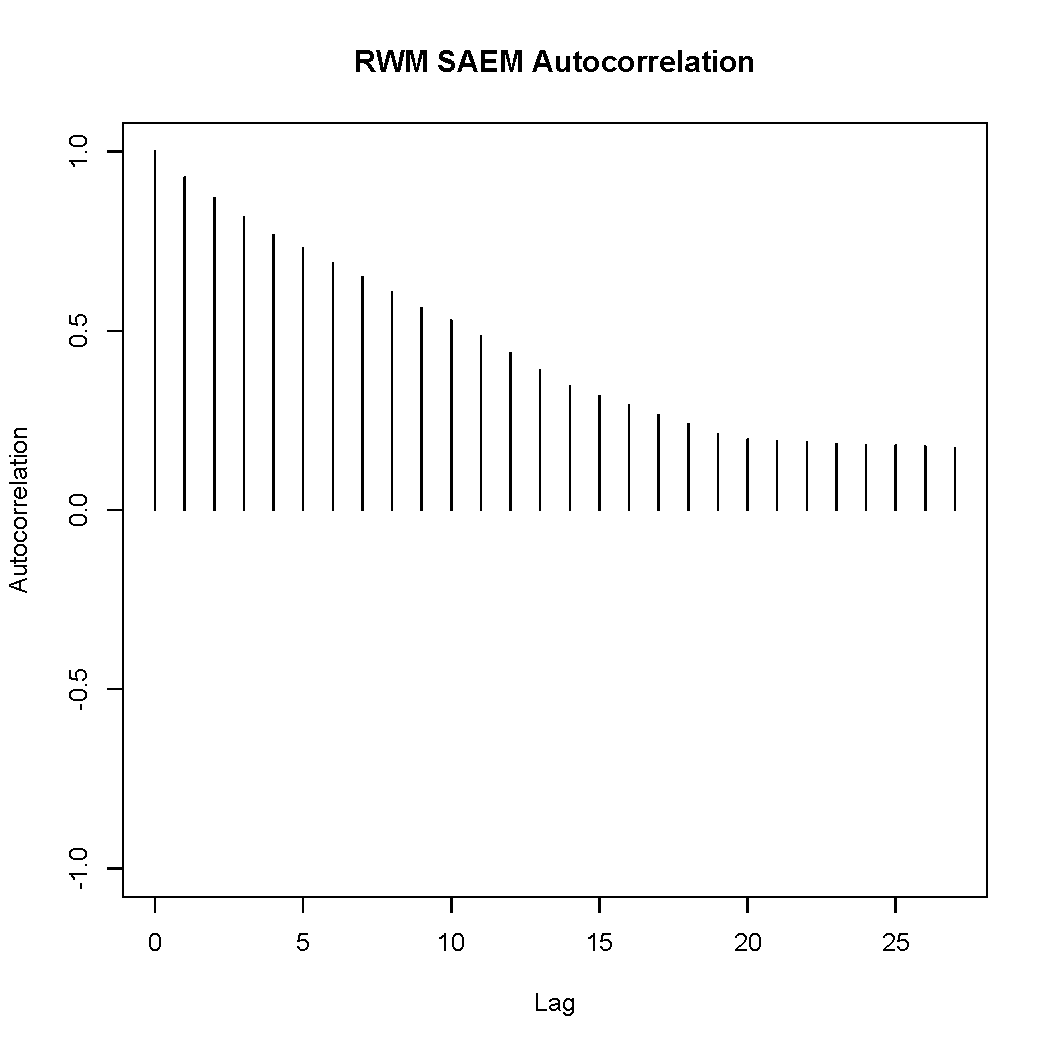
\includegraphics[scale=0.2]{rwm_autocorr.pdf}
      \begin{center}
      \caption{RWM}
      \end{center}
    \end{column}%
    \hfill%
    \begin{column}{.30 \textwidth} % Right column and width
      
      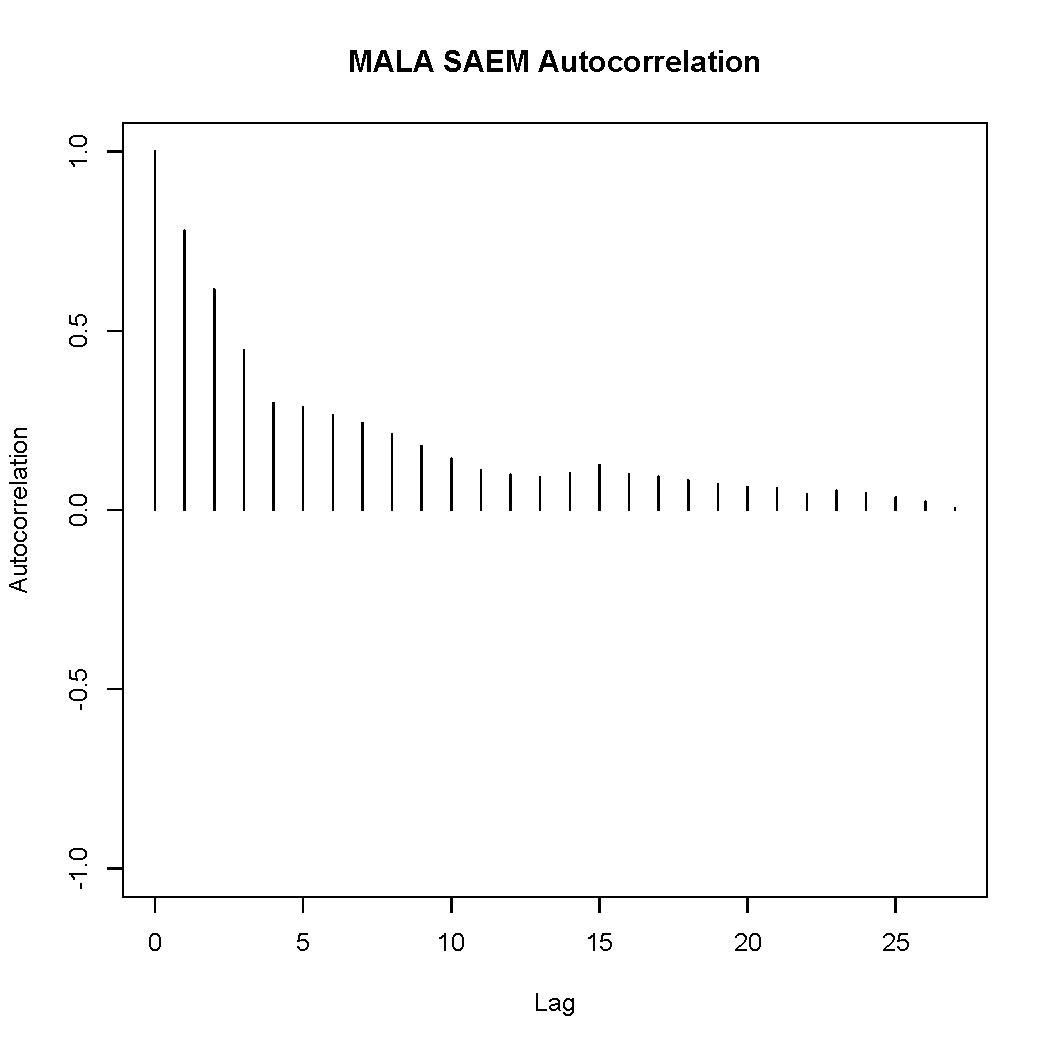
\includegraphics[scale=0.2]{mala_autocorr.pdf}
      \begin{center}
      \caption{MALA}fa
      \end{center}
    \end{column}

    \begin{column}{.30 \textwidth} % Right column and width
      
      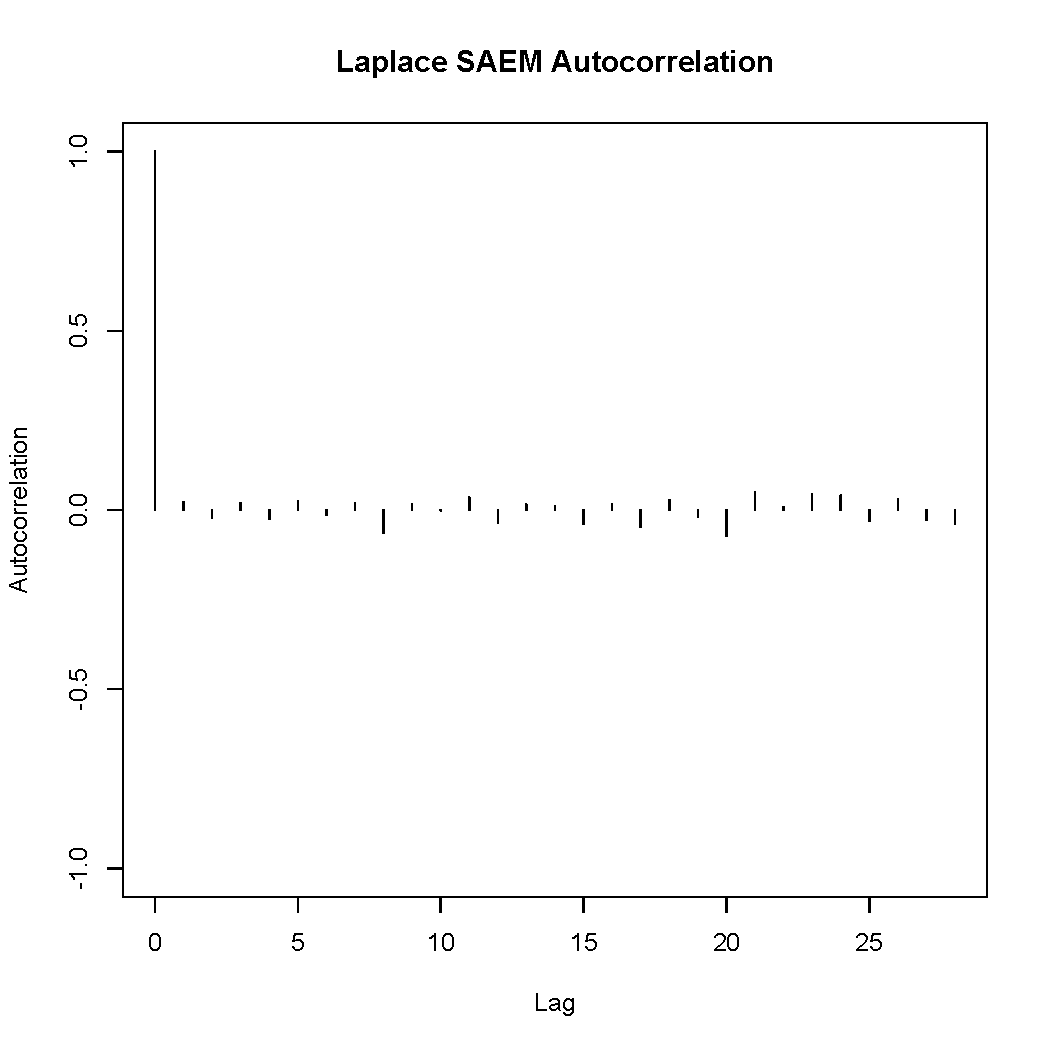
\includegraphics[scale=0.2]{laplace_autocorr.pdf}
      \begin{center}
      \caption{Laplace}
      \end{center}
    \end{column}
  \end{columns}

\end{frame}

\begin{frame}
\frametitle{PK-PD datasets}

We use a Linear Plateau model here and the the structural model is:
\begin{equation}
    f(z_i)= 
\begin{cases}
    (Y_{max})_i + B_i*(t_i-(X_{max})_i) ,& \text{if } t\geq (X_{max})_i\\
    (Y_{max})_i,              & \text{otherwise}
\end{cases}
\end{equation}
Where $z_i=((X_{max})_i,(Y_{max})_i,B_i)$.


\begin{figure}[h]
\begin{center}
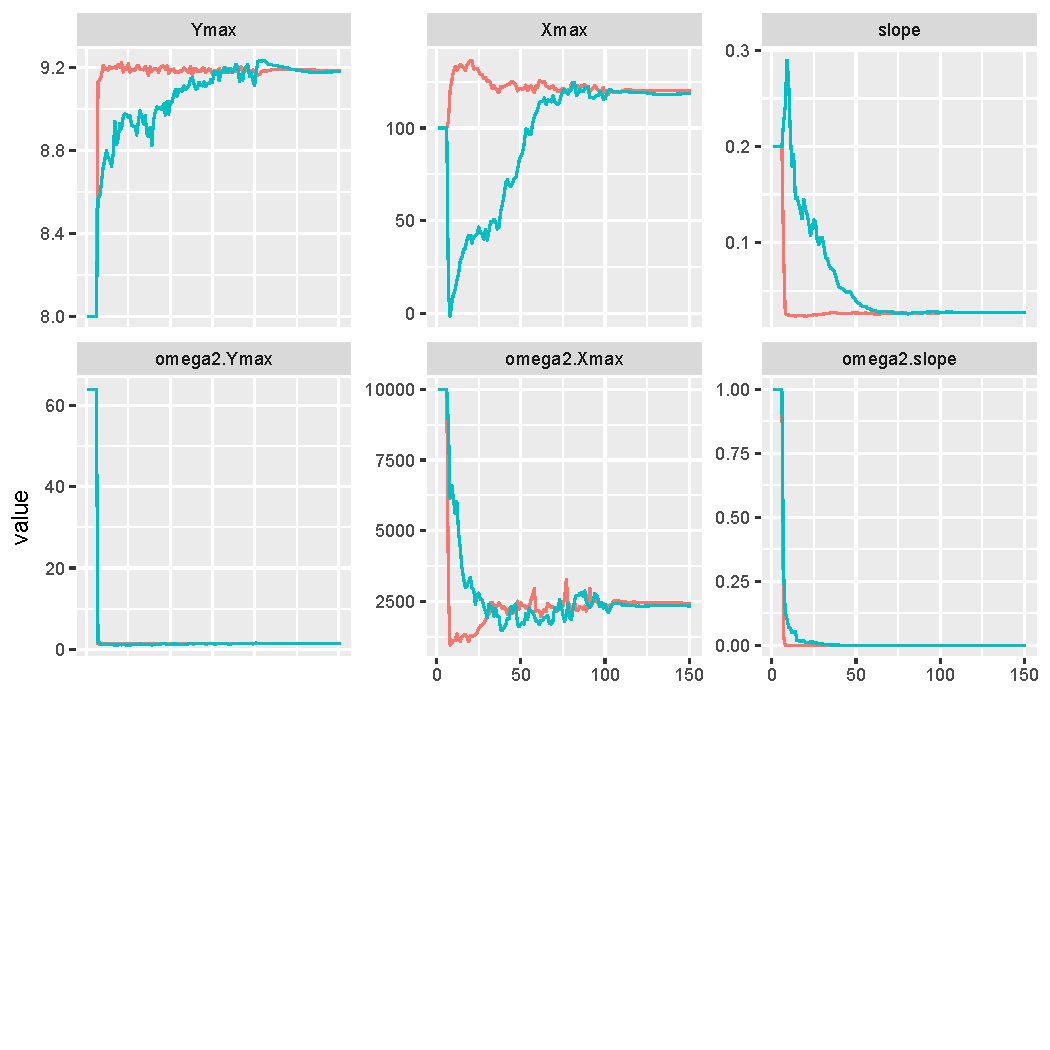
\includegraphics[scale=0.3]{map.pdf}
\end{center}
\caption{Estimate of $X_{Max}$ for 100 replicates}
\end{figure}

\end{frame}



\begin{frame}{}
  \centering \Large
  \emph{Thank you}
\end{frame}


\end{document}
